\begin{frame}
	\titlepage 
\end{frame}


\section{Contexte}

\subsection*{}
\begin{frame}{\insertsectionhead}
\vspace{-0.2cm}
		\begin{columns}
			\column{0.5\textwidth}
			\centering
			\begin{figure}
				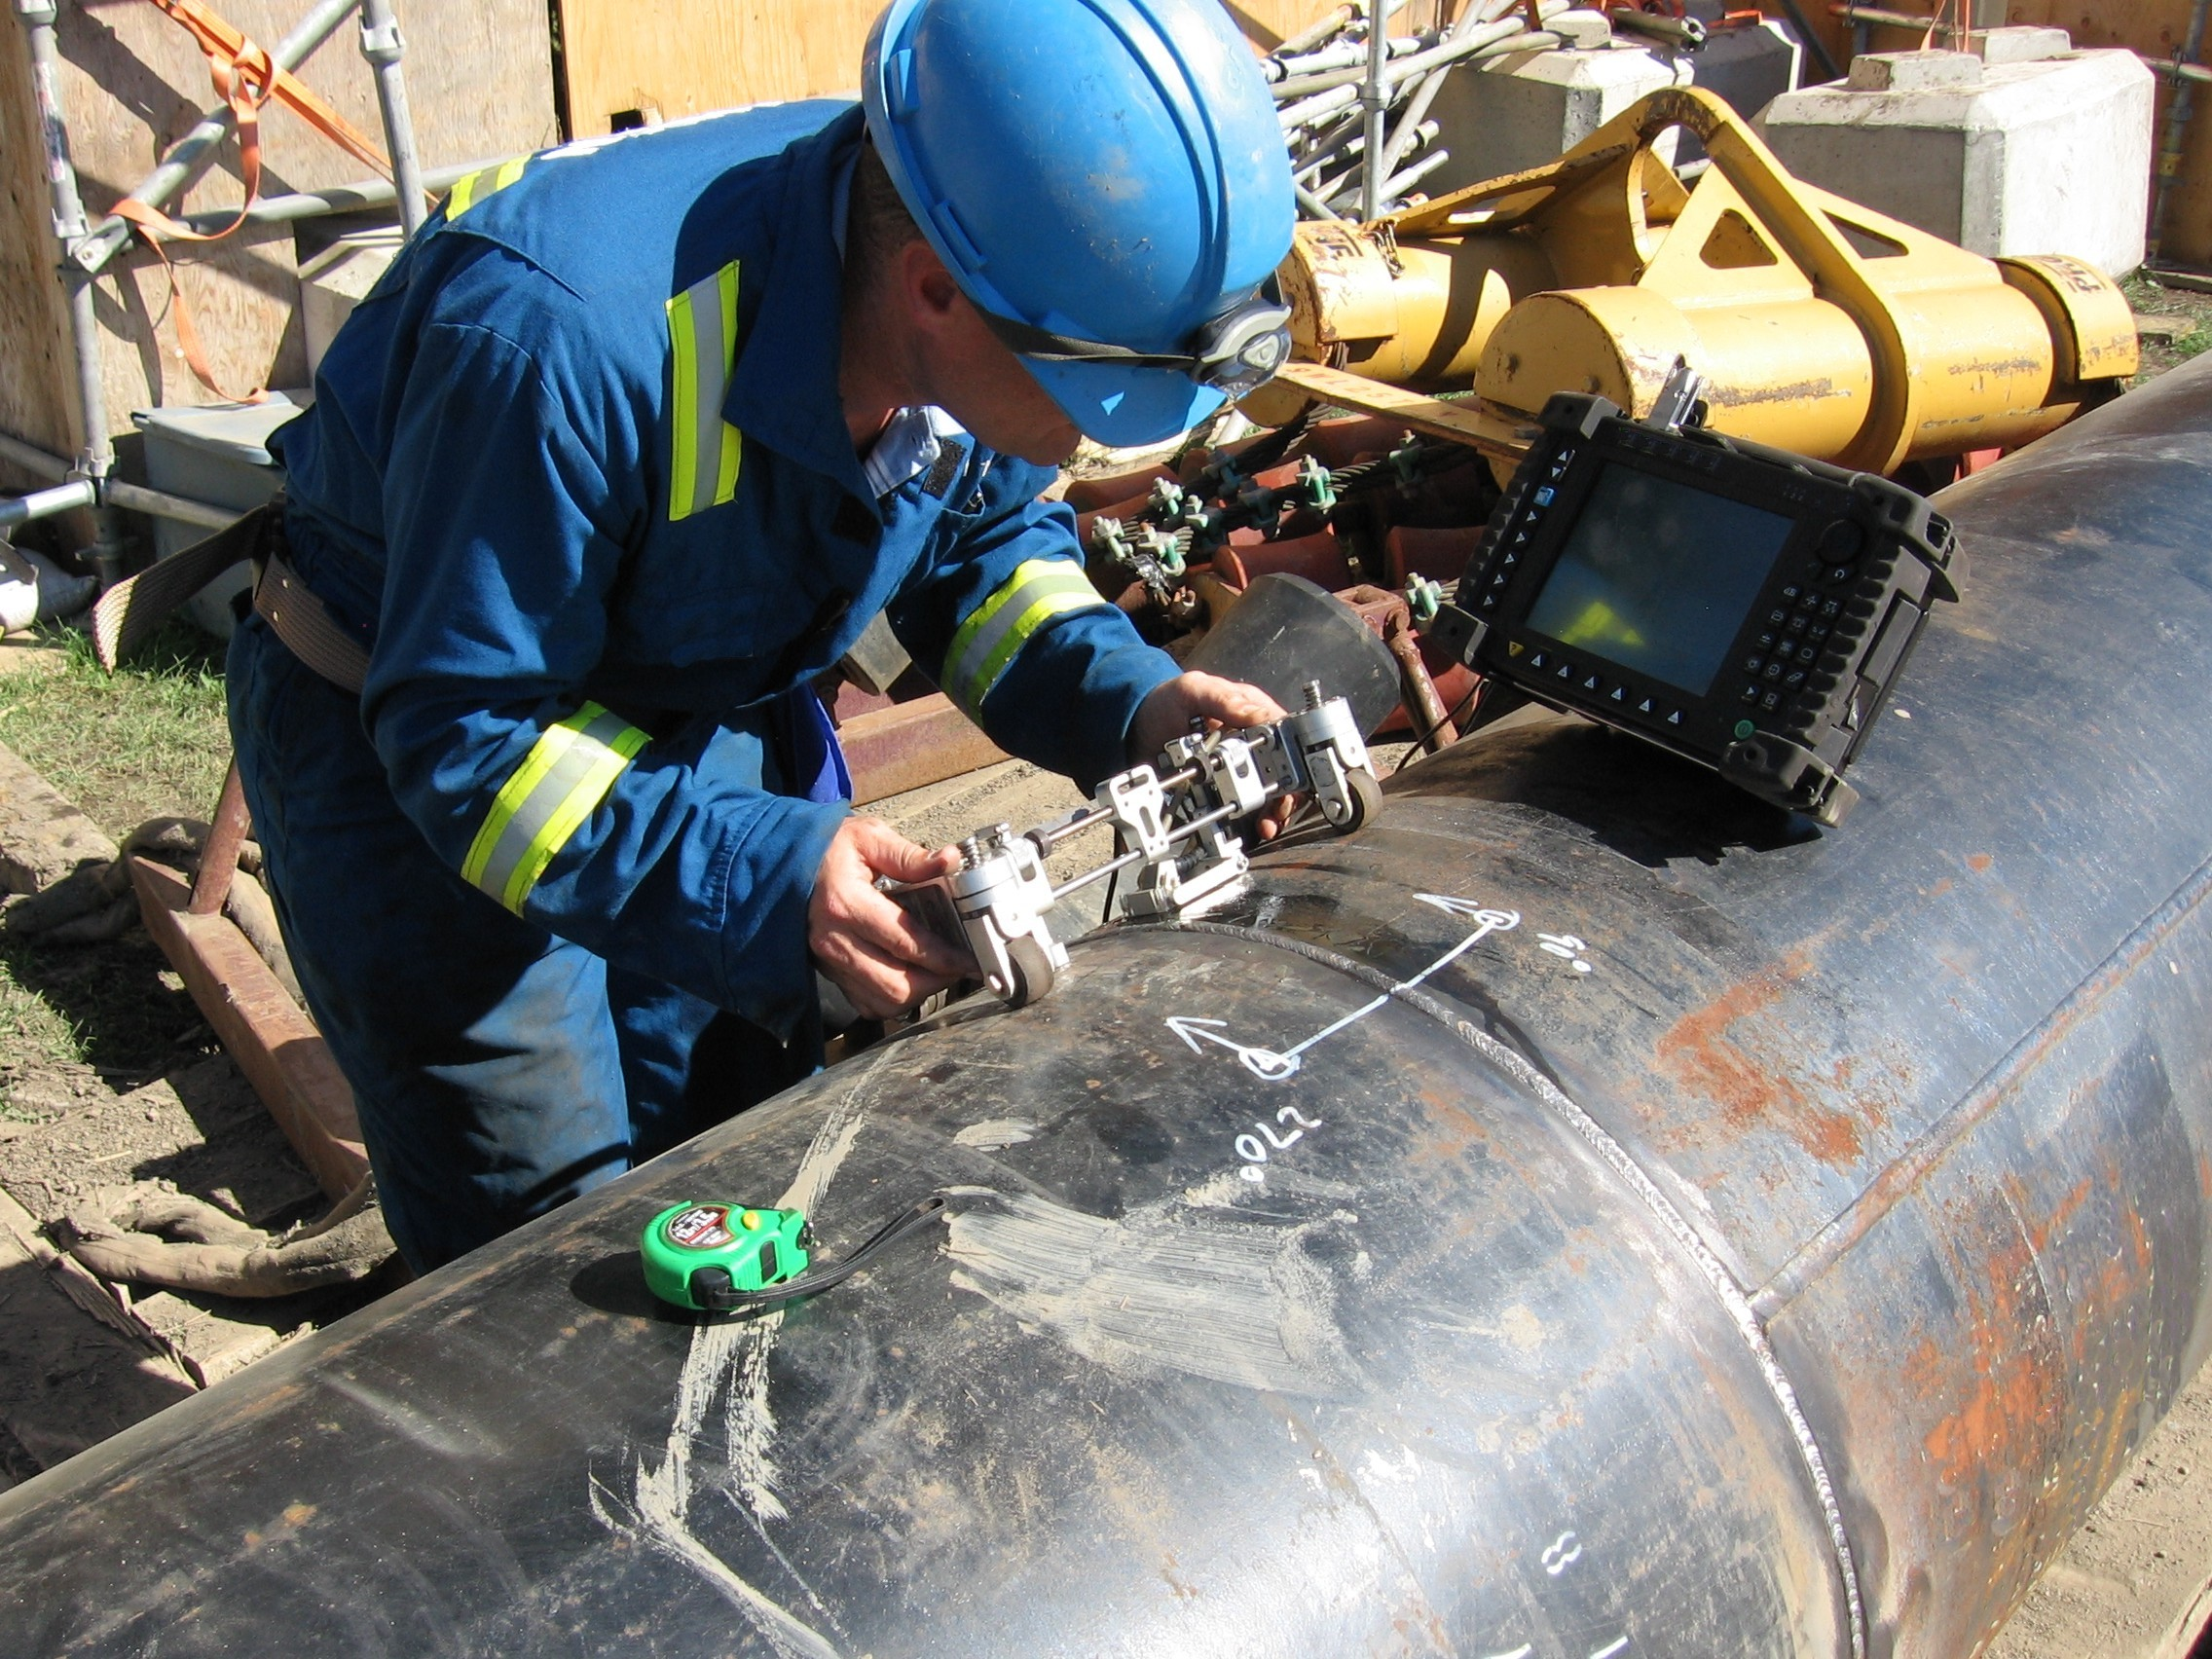
\includegraphics[height=3cm]{img/us_test.jpg}\\
				{\tiny{\raggedright \itshape Image Davidmack}\\ \centering \scriptsize{Contrôle sur pipeline}}
			\end{figure}		
			\column{0.5\textwidth}
			\begin{figure}
				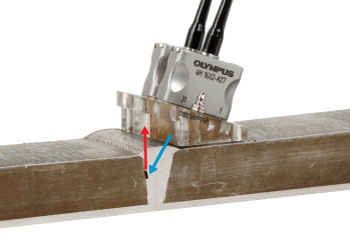
\includegraphics[height=3cm]{img/olympus.jpg}\\
				 {\tiny{\itshape Image Olympus}\\ \centering			\scriptsize{Exemple de test en réflexion}}
			\end{figure}
		\end{columns}	
		\vspace{0.4cm}	

	%\begin{columns}
			%\column{.5\textwidth}
			Contrôle et évaluation de soudures :\\
			\begin{itemize}
				\item de centrales nucléaires (système de refroidissement)
				\item de pipelines 
			\end{itemize}
			%\column{.05\textwidth}
			%\ding{222}
			%\column{.45\textwidth}
			%\centering
			\vspace{-0.4cm}
			\begin{columns}
			\column{0.7\textwidth}
			\centering
 			\indent \ding{222} porosité, fissure, manque de fusion, corrosion, corps étrangers,\ldots
 			\column{0.3\textwidth}
 			\centering
 			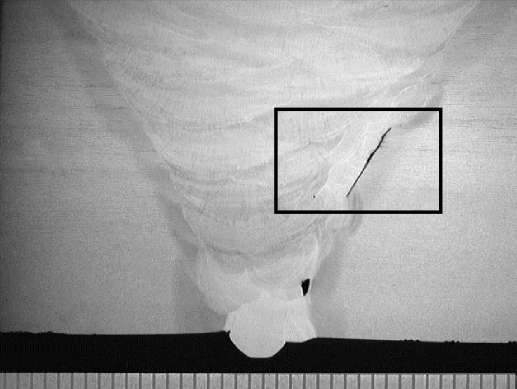
\includegraphics[width=0.95\textwidth]{img/defaut_soudure.png}\\
 			{\itshape \tiny Image extraite de Consonni et al., \\[-0.2cm]Insight, 2011}
 			\end{columns}
	%\end{columns}
\end{frame}


\subsection*{}
\begin{frame}{\insertsectionhead}
\begin{small}
\vspace{-0.5cm}
\hspace{1cm}
\onslide<2->{
\begin{picture}(0,0)(0,0)\put(50,5){
		\textcolor{red}{Forte anisotropie imprévisible}
}\end{picture}
}
	\begin{columns}[c]
			\column{.5\textwidth}<1->
			\centering
			\begin{figure}
				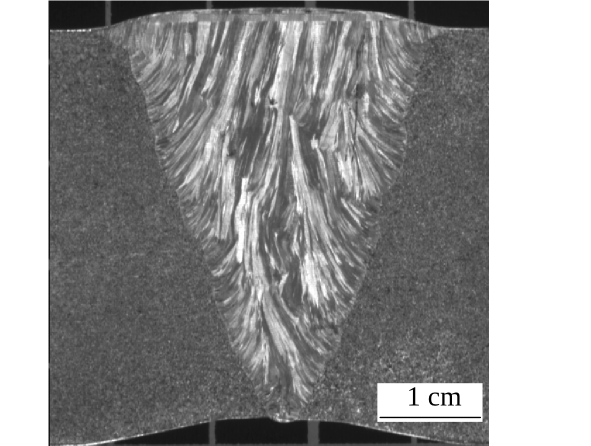
\includegraphics[height=2.7cm]{./img/soudure1.png}\\
				{\tiny{ \itshape Image extraite de Chassignole, 2010} \\ \centering \scriptsize Macrographie d'une soudure austénitique  }
			\end{figure}
			\column{.001\textwidth}<2->
			\hspace{-2.8cm}
			\vspace{2.5cm}
			\begin{tikzpicture}
					\draw[<-, thick,shorten <=2pt,shorten >=2pt,red] (-1.5,3)--(0.0,4.6);
			\end{tikzpicture}
			\column{.9\textwidth}<2->
			%\vfill
			\hspace{-1cm}
			$\hookrightarrow$ déviation et division du faisceau ultrasonore\\[0.2cm]
			\hspace{-0.5cm}
			\hspace{1cm}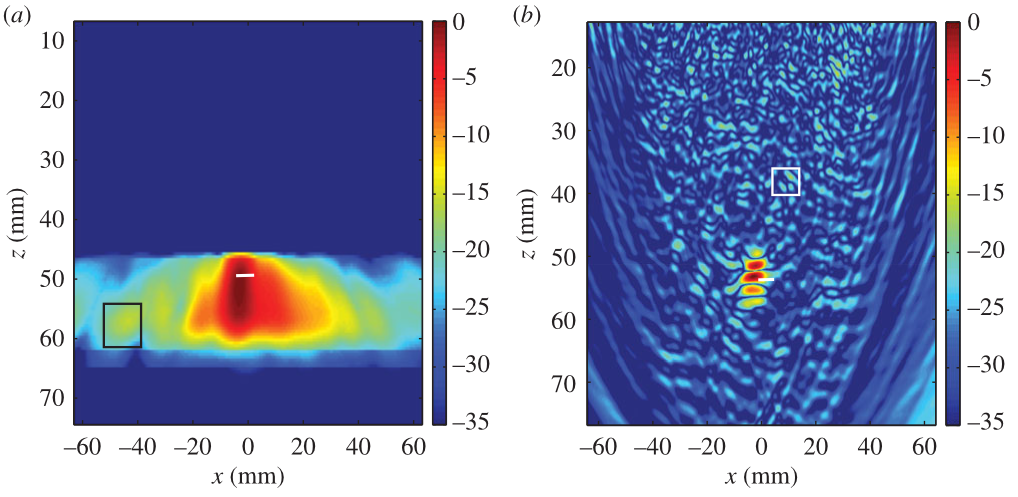
\includegraphics[height=2.5cm]{img/tfm_dort.png}\\
			{\tiny{ \itshape Images extraites de Cunningham et al., Proc. R. Soc., 2016} \\[0.2cm] \hspace{1cm} \scriptsize Méthodes DORT (gauche) et FTP (droite)\\[-0.1cm] \hspace{1.5cm}sur modèle EF de soudure anisotrope }
				
	\end{columns}
	%\vspace{0.3cm}
	\begin{columns}[c]
			\column{.5\textwidth}<1->
			%\begin{block}{}
				\begin{itemize}
					\item[$\bullet$] méthodes par sommation cohérente des signaux (ex : FTP)
					\item[$\bullet$] Décomposition des matrices de covariance (ex : DORT)
				\end{itemize}
			%\end{block}
			\column{.05\textwidth}<2->
			\ding{222}
			\column{.5\textwidth}<2->
				\begin{itemize}
					\item[\ding{55}] requièrent une connaissance\\ \emph{a priori} de la vitesse\\
					\item[\ding{55}] sujettes aux artefacts
				\end{itemize}
	\end{columns}
	\vspace{0.1cm}
	\begin{columns}[c]
		\column{.5\textwidth}<3->
			\begin{itemize}
				\item[$\bullet$] Résolution d'un problème d'optimisation
			\end{itemize}
		\column{.05\textwidth}<3->
			\ding{222}
		\column{.5\textwidth}<3->
			\begin{itemize}
			\item optimisation topologique :\\\hspace{-0.5cm}\small{\emph{Dominguez et al.}, \emph{Rodriguez et al.}}\\[0.1cm]
			\item[\ding{51}] {reconstruction d'un ensemble de paramètres : FWI}
		\end{itemize}		
	\end{columns}
\end{small}
\end{frame} 


\section{La FWI}
\subsection*{}
\begin{frame}{La Full Waveform Inversion}
	\begin{columns}
		\column{0.6\textwidth}<1-1>
		\begin{itemize}
			\item Développée pour la géophysique\\[0.3cm]
			\item Estimation des paramètres élastiques\\ $~~~~~~\hookrightarrow$ optimisation locale\\[0.3cm]
			\item Utilise tout le champ d'onde\\[0.3cm]
		\end{itemize}
		
		\column{0.6\textwidth}<2->
		\begin{itemize}
			\item<2-> Fonction de coût : $C(\bm{m})=\frac{1}{2}||\bm{d}_{obs}-\bm{d}_{cal}(\bm{m})||^{2}$\\♥
			\item<3-> Optimisation locale : modèle optimal quand $C'(\bm{m})=0$
			\item[$\hookrightarrow$]  \\[0.5cm]
			\item \only<3->{Perturbation du modèle : $\bm{\Delta m}=-(C'')^{-1}$\fcolorbox{white!0}{white!0}{$C'$}} \onslide<2->{Perturbation du modèle : $\bm{\Delta m}=-(C'')^{-1}$\fcolorbox{DeepSkyBlue4}{white!0}{$C'$}}
%	\end{itemize}
		
		
		\column{0.5\textwidth}<1->
		\begin{figure}
			\centering
			\hspace{-0.3cm}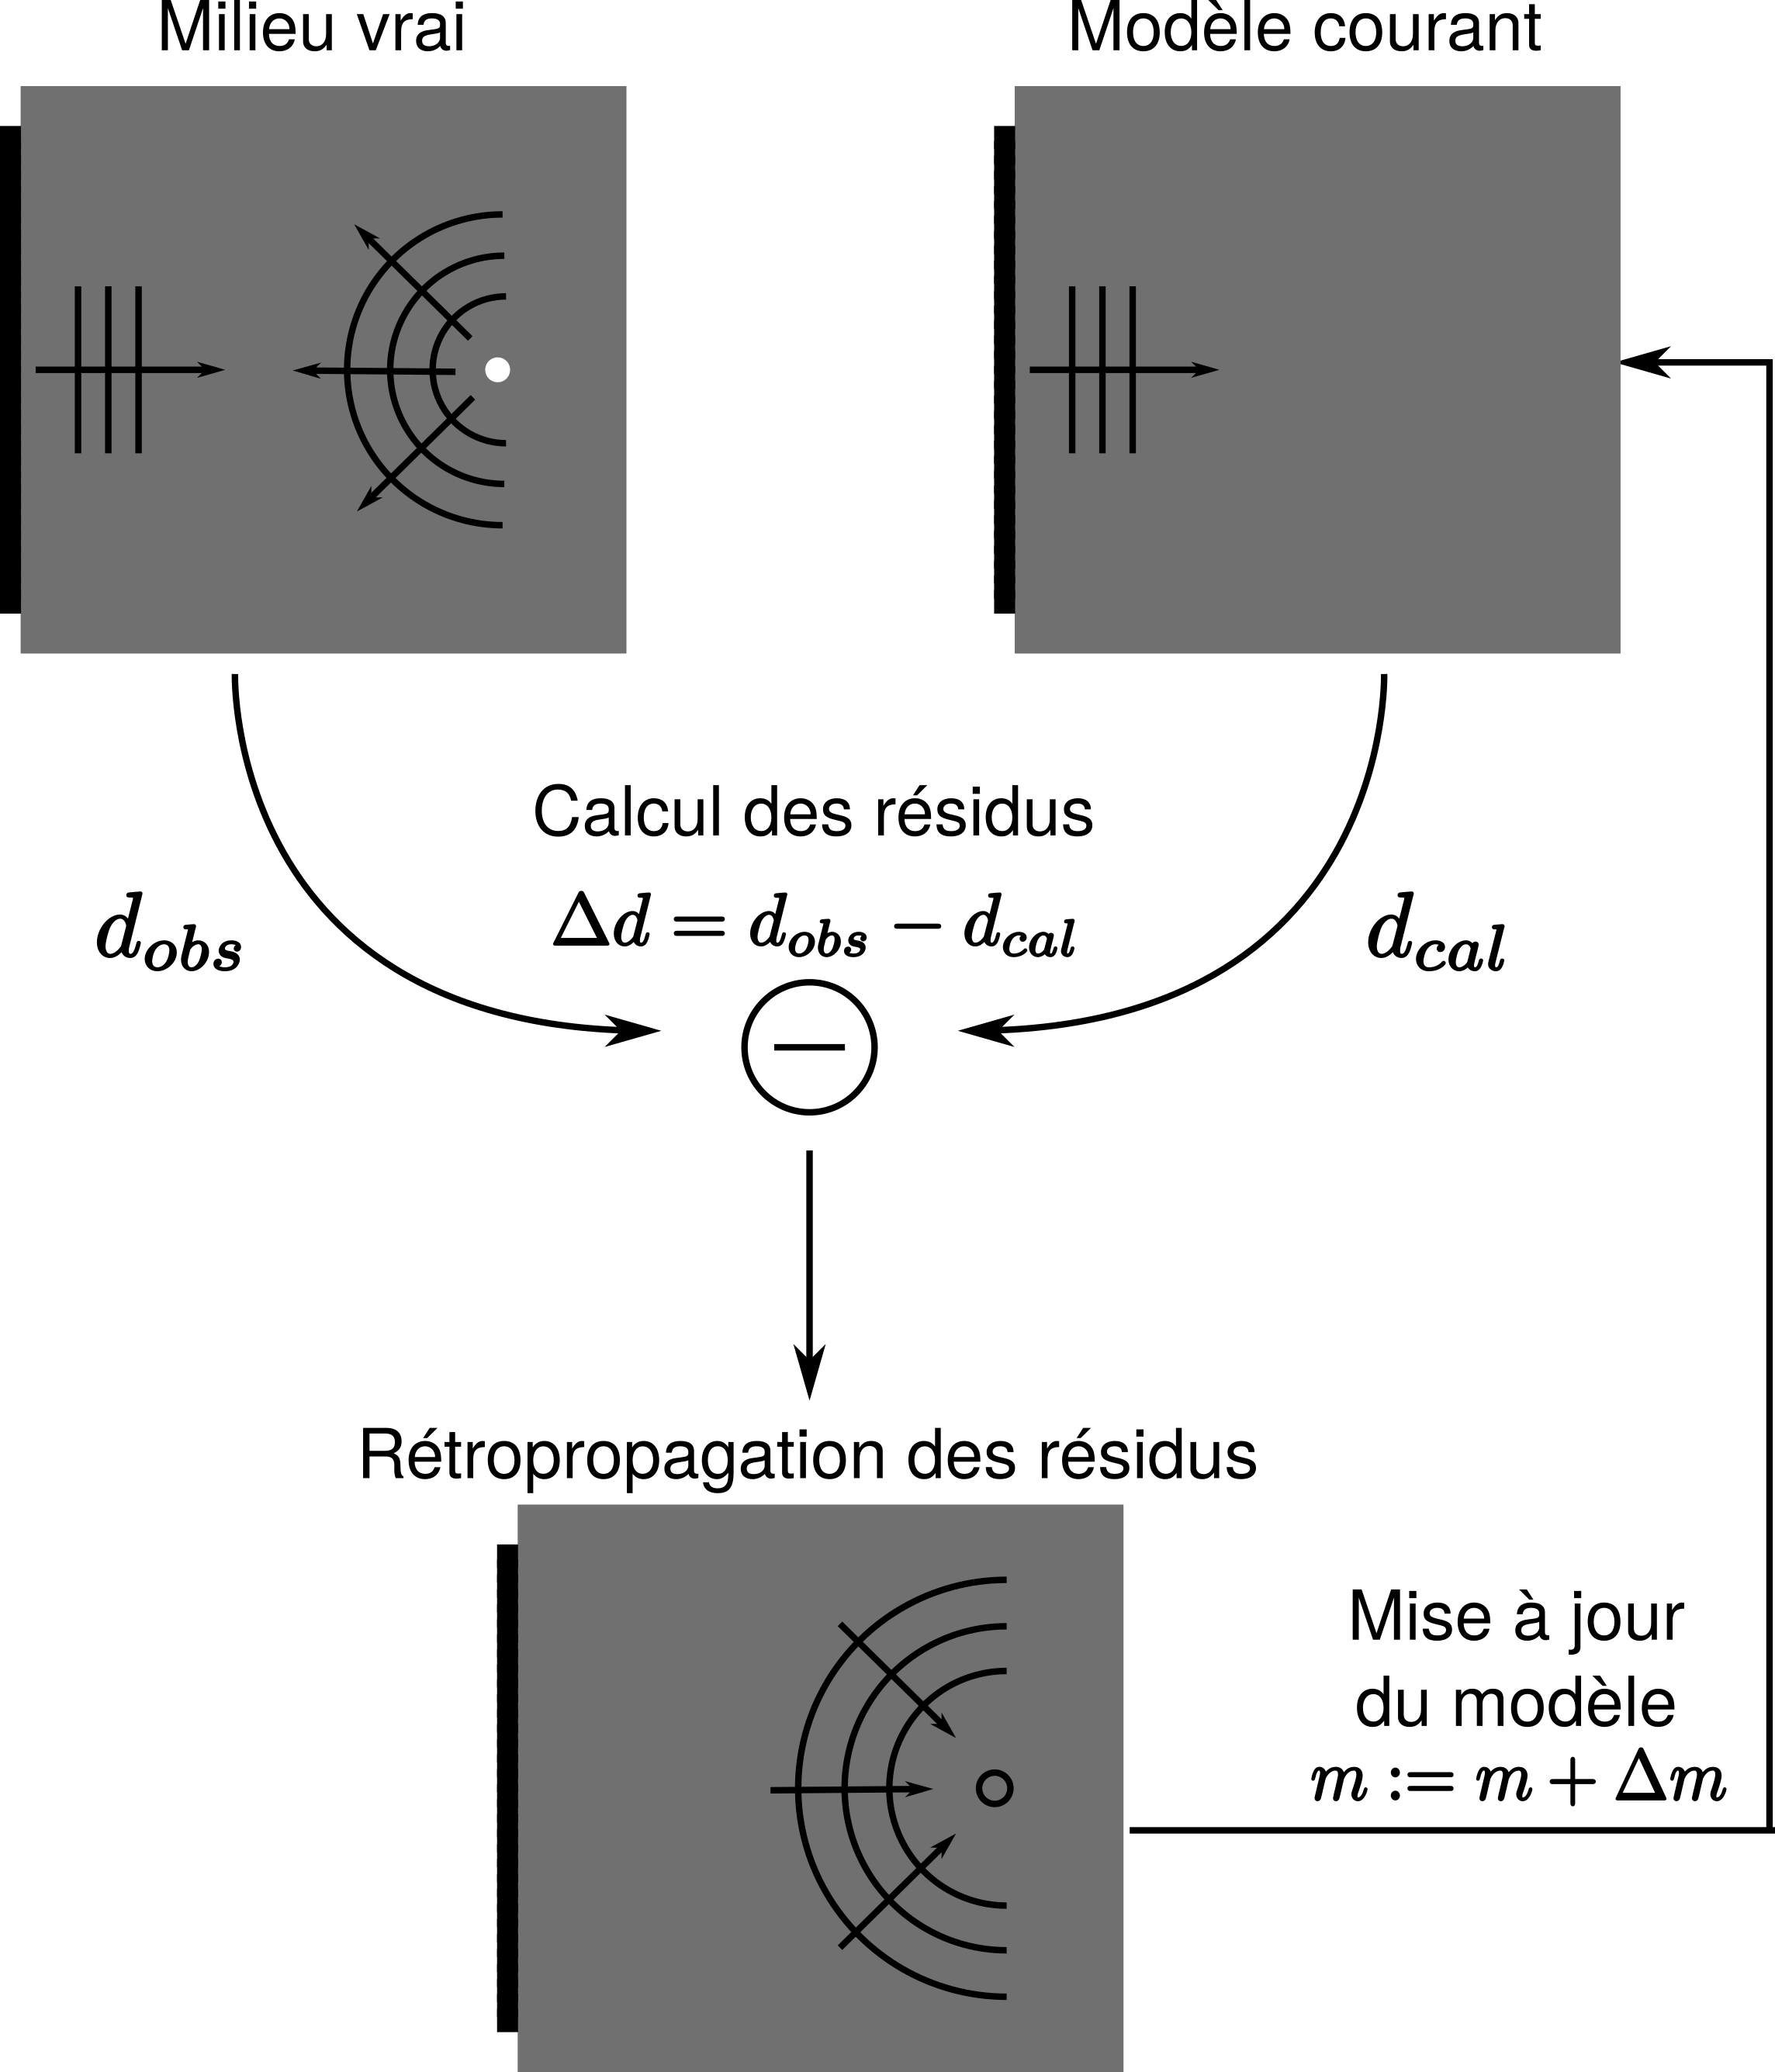
\includegraphics[width=\textwidth]{img/schema_fwi2.png}
		\end{figure}
	\end{columns}
	
\end{frame}


